\chapter{Theory}
\label{ch:theory}

\emph{Write an intro to the chapter}.

\section{Instruments}
\label{sec:instruments}

The data in this project was aqcuired in an SEM with an EDS detector, which both are described in this section.


\subsection{SEM}
\label{theory:instruments:sem}

This subsection about SEM is based on Goldstein \cite{goldstein_scanning_2018}.

Scanning electron microscopes provide a high spatial resolution of micro- and nanoscale features.
The features revealed can be size, composition, shapes, topology, crystallography, and other chemical and physical properties. % Kinda copied from Goldstein p. VII
The working principle of an SEM is based on the interaction of a finely focued beam of electrons with the sample, where the beam is scanned over the sample surface to create a 2D image.
The interactions between the beam and the sample produce multiple signals, both as electrons and photons, which provide different information about the sample.
Auger electrons and secondary electrons give information about the surface of the sample, while backscattered electrons and X-rays give information about the composition of the sample.
The signals are not only created at the surface, but also inside the sample, and the region where the signals are created is called the interaction volume.

% The inteaction volume
After the interaction and creation of a signal, the signal must escape the sample to be registered by a detector.
The escape depth of the signal types is illustrated in \cref{fig:interaction_volume}.
When a signal is formed inside the sample, the signal can both be absorbed or scattered within the sample.
The signals with low energy are absorbed, and will thus only be emitted at the surface, e.g. Auger electrons and secondary electrons.
The signals which originate from deeper inside the sample, e.g. backscattered electrons and X-rays, can interact with the sample multiple times before they are emitted and detected.

% figures/interaction_volume.png
\begin{figure}[ht]
    \centering
    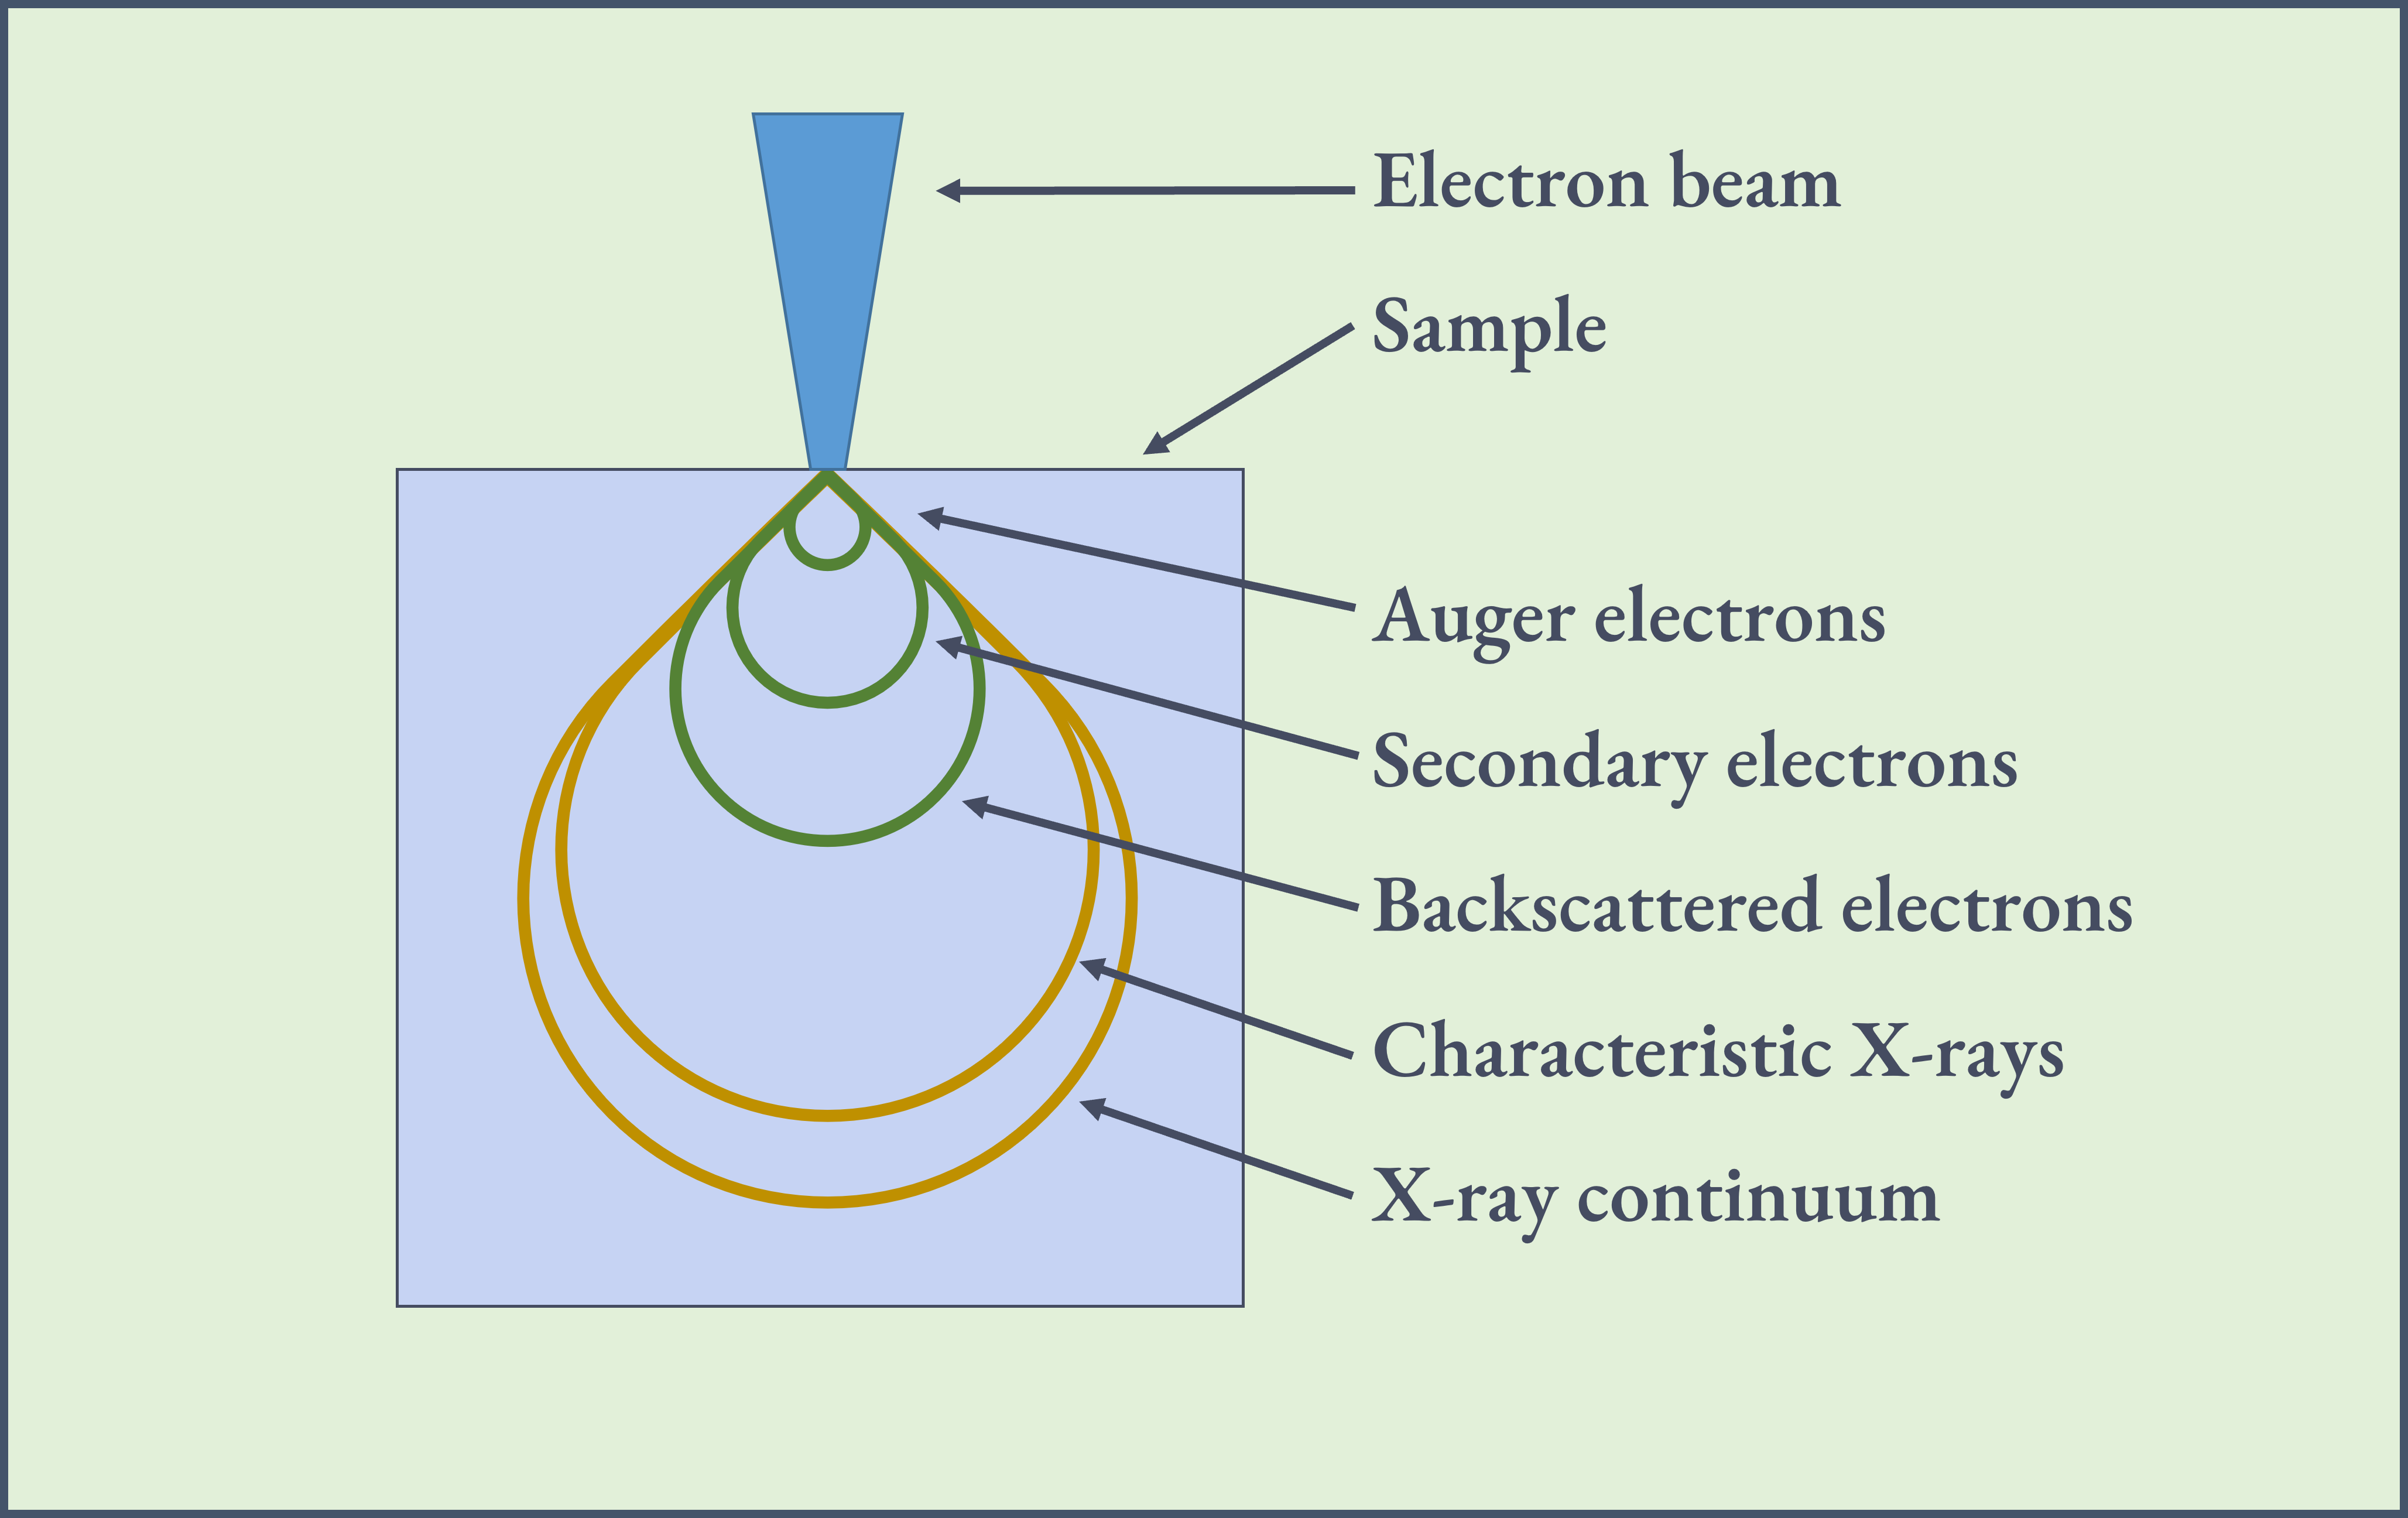
\includegraphics[width=0.8\linewidth]{figures/interaction_volume.png}
    \caption{
        Illustration of the interaction volume of the different signals.
        The signals are emitted in all directions, which is why the interaction volume is spherical.
        The blue signals are electrons and the orange signals are X-rays.
        The depths are not to scale.
    }
    \label{fig:interaction_volume}
\end{figure}


\ton{Do you want me to write about the different signals, ie. SE and BSE?}


% The parts in the SEM
An SEM consists of several parts, which are illustrated in \cref{fig:SEM_setup}.
The electron gun is the source of the electrons.
The condenser lens focuses the electrons to a small beam.
The two apertures sets the size of the beam, which is important since the electrons closest to the central axis of the beam have fewest aberrations.
The scanning coils are used to scan the beam over the sample in the raster fashion.
The objective lens focuses the beam to a small spot on the sample.
In general a smaller spot allows higher resolution, because the signal is recorded from a smaller area.
However, this effect is limited by several factors, such as the interaction volume.
The detectors are placed above the sample.

\ton{What more do you want me to write about the SEM?}

% figure/SEM_setup.png
\begin{figure}[ht]
    \centering
    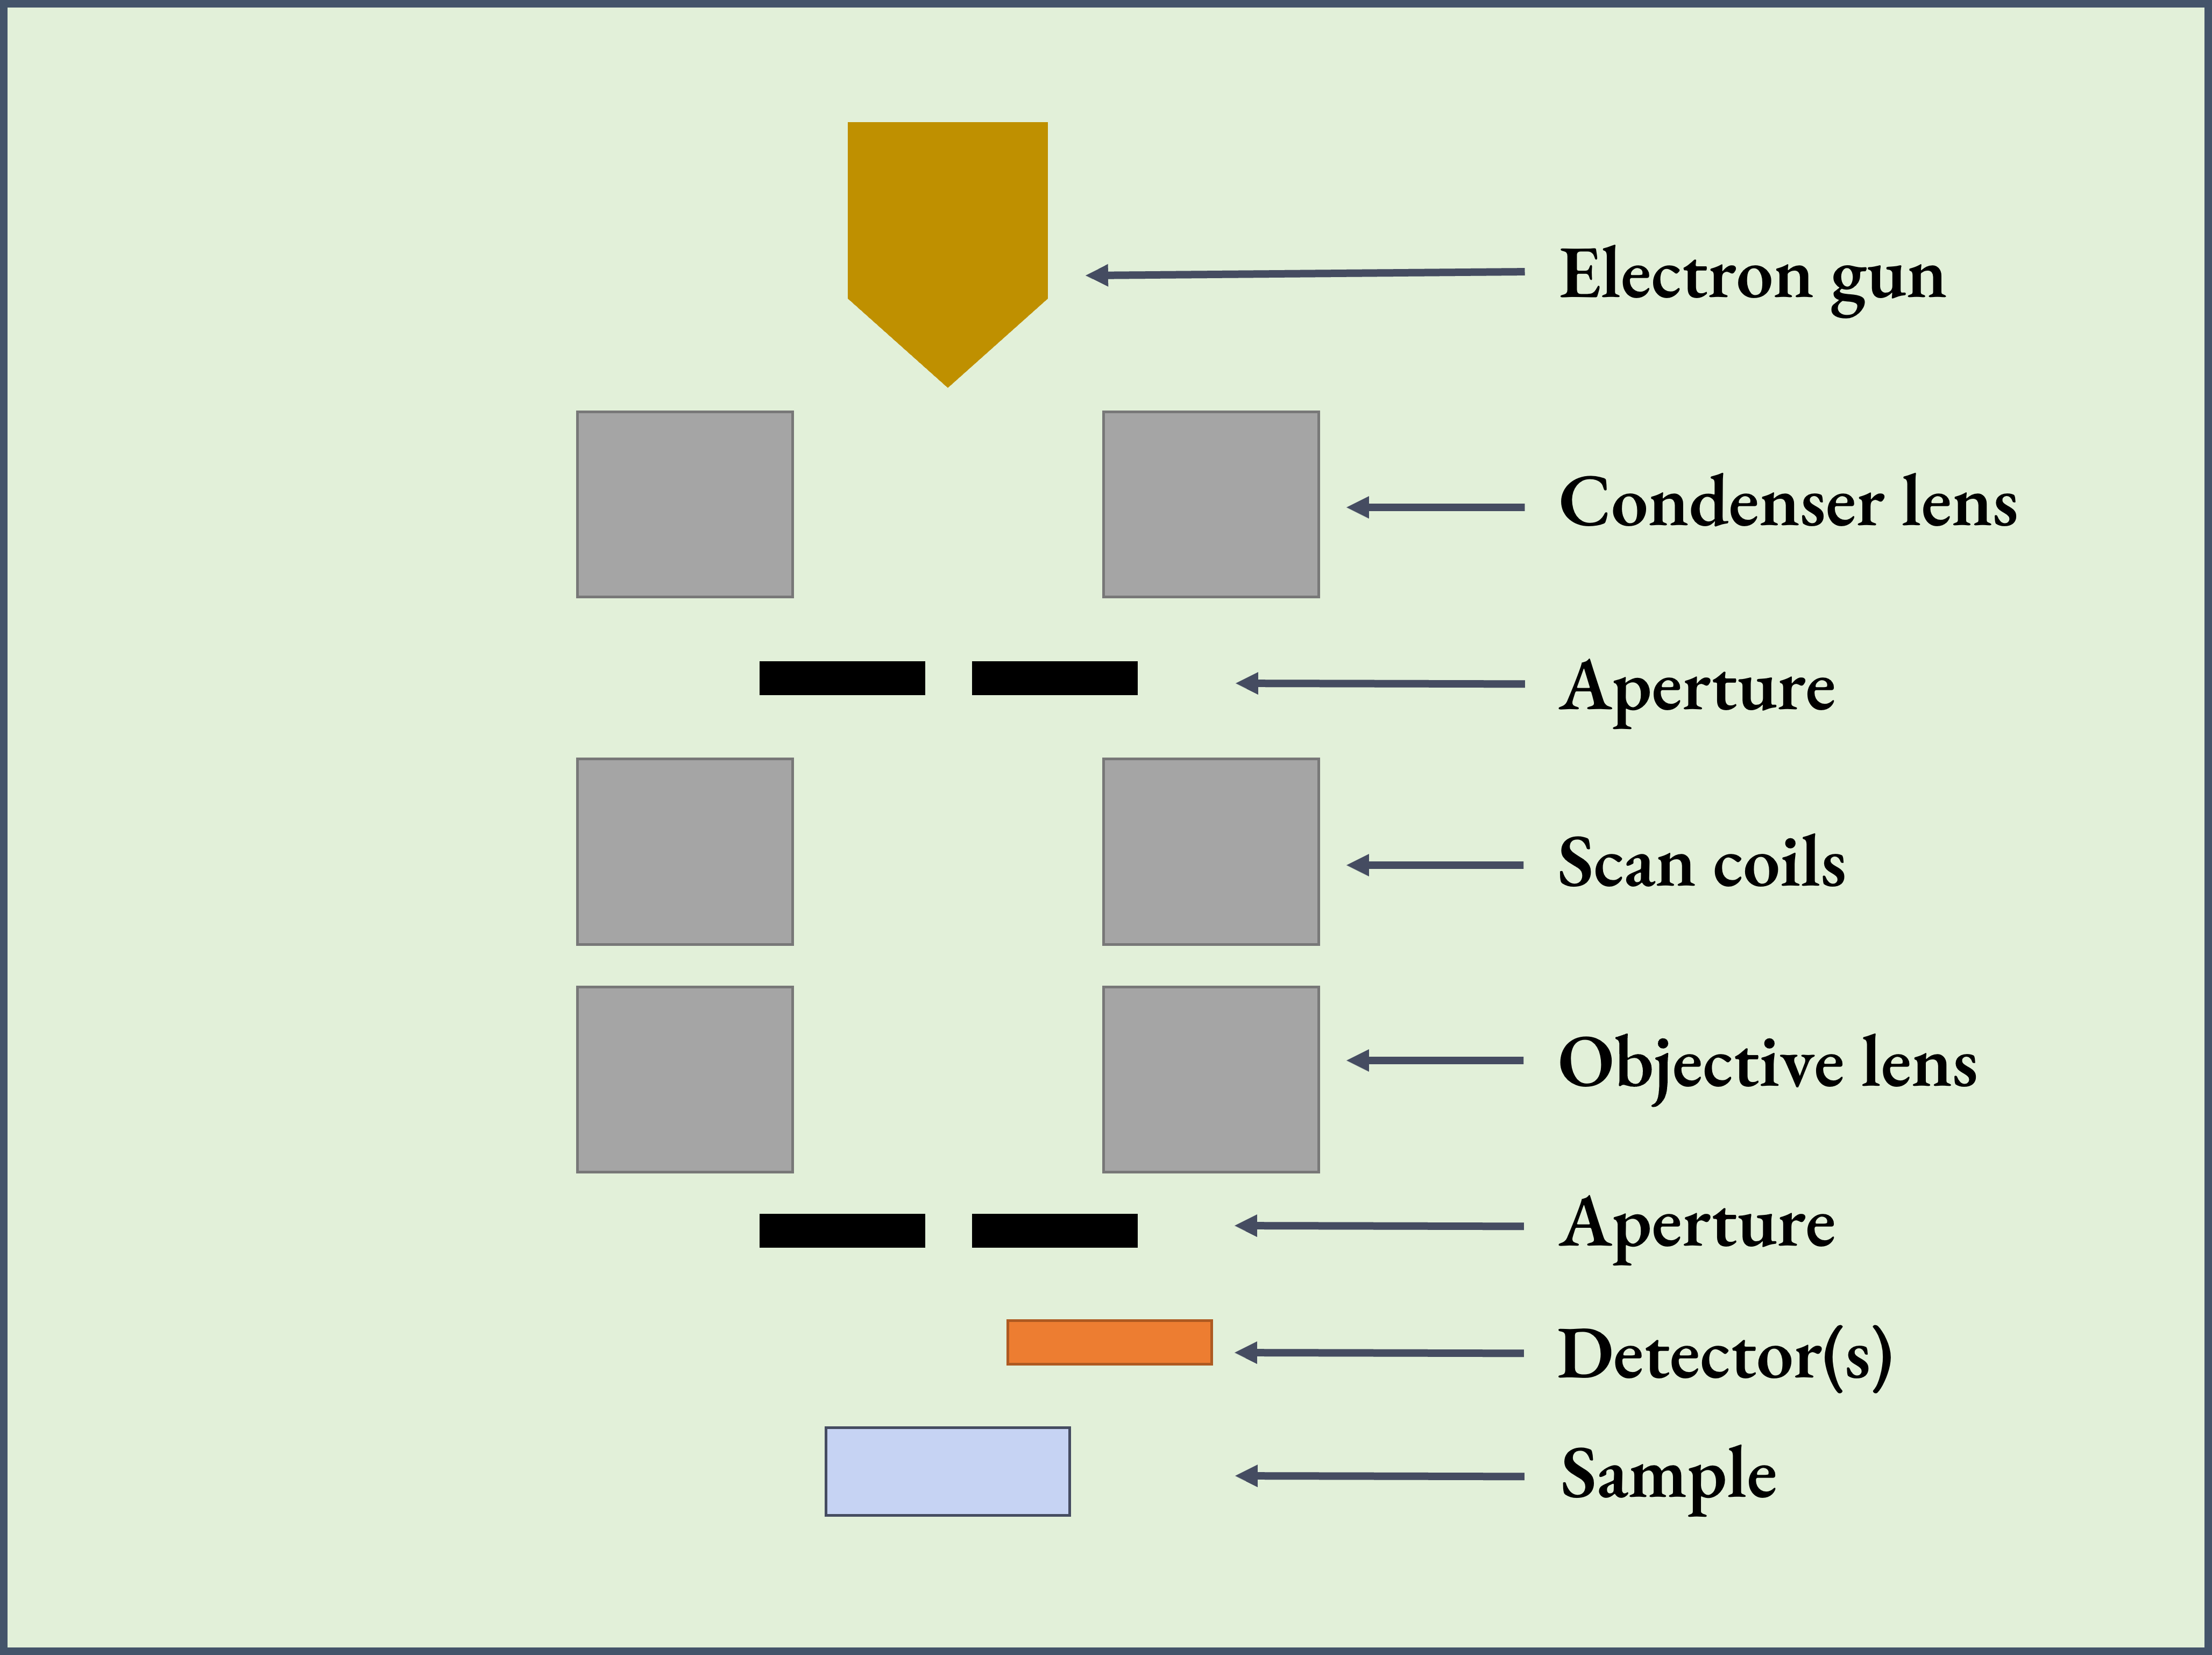
\includegraphics[width=0.8\linewidth]{figures/SEM_setup.png}
    \caption{
        Illustration of the parts in an SEM.
    }
    \label{fig:SEM_setup}
\end{figure}